\chapter[Planificación]{
  \label{chp:plan}
  Planificación
}
\minitoc
\newpage

Neste capítulo explicarase a planificación do traballo realizado e a avaliación de custes.  

\section{Orixe do proxecto}

Produciuse un encontro informal con membros de Cuac FM (a radio comunitaria da Coruña) e a URCM onde se entrou en contacto cos usuarios finais do proxecto a realizar. A URCM (Unión de Radios Comunitarias de Madrid) está composta por unha serie de emisoras independentes e con programas de seu; todos eles listados nunha sección da web (ver figura \ref{fig:urcm}) que á súa vez da acceso ao directorio dos ficheiros de audio (aos que a partir de agora nos referiremos coma \say{audios}) publicados por ditas emisoras. Esta sección da web, pese a súas limitacións, leva funcionando uns anos e resultou ser moi positiva para a redifusión dos programas por distintos colectivos.

\begin{figure}[h]
	\centering
	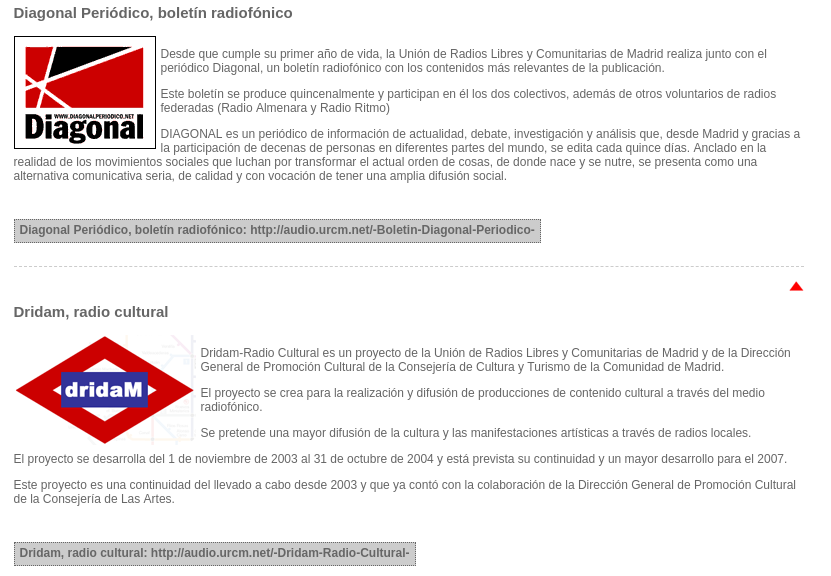
\includegraphics[scale=0.55,keepaspectratio=true]{./images/urcm.png}
	\caption{Sección de audios da web da URCM que inspira o proxecto.}
	\label{fig:urcm}
\end{figure}

Inspirados nesta idea, propúxose crear unha ferramenta semellante, esta vez para a ReMC (Red de medios comunitarios), unha federación de medios comunitarios do Estado Español. Definíronse uns requirimentos iniciais, máis centrados naquel entón na
redifusión e a organización que na escoita.

A seguinte lista é unha transcrición das notas tomadas durante ese encontro:

\begin{itemize}
	\item Os usuarios dos sistema son as propias emisoras.
	\item As emisoras teñen que poder engadir audios.
	\item As emisoras poden acceder aos audios das outras.
	\item As emisoras teñen que poder saber quen está a emitir os seus programas.
\end{itemize}


\section{Iteracións}

Como se explicou no capítulo \ref{chp:metodoloxia}, o desenvolvemento executouse de  de forma iterativa e incremental onde unha iteración son os obxectivos a cumprir entre dúas reunións co cliente. Ao ser isto un proxecto de final de carreira, contarase o tempo entre as sesións de revisión de progresos entre o director do proxecto e o alumno. Estas reunións tiveron unha periodicidade bisemanal na súa meirande parte, reducindo a duración dos ciclos nas derradeiras fases da implementación.


\subsection{Primeira reunión (Iteración 0)}

Na primeira reunión estableceuse a lista de obxectivos xerais do proxecto repasados xa na sección \ref{obxectivos}. Estes supoñen unha aproximación ao problema máis ambiciosa que a idea orixinal de ter un simple directorio web compartido entre emisoras pois ten en conta as necesidades dos ouvintes e a propiedade dos programas por parte dos seus autores e non necesariamente da emisora, cousa bastante común no mundo da radio comunitaria. Foi neste momento cando se tomou a decisión de utilizar Django coma framework de desenvolvemento e PostgreSQL coma sistema de xestión de bases de datos.

Os obxectivos de cara a primeira iteración foron:

\begin{itemize}
	\item Facer un primeiro borrador do deseño do modelo de datos.
	\item Investigar a manipulación de ficheiros RSS utilizando Python. Desde o principio, a consulta dos ficheiros de RSS intuíuse coma o xeito de manter actualizados os programas mais neste momento aínda non se tomara unha decisión firme de como facelo.
\end{itemize}

\subsection{Iteración 1}

Cumpríronse os obxectivos marcados, entregando un deseño preliminar do modelo de datos na data estimada. No diagrama da figura \ref{fig:classold} vese que o modelo aínda era alleo aos requisitos de Django que se explicarán máis adiante no capítulo \ref{chp:disenho} sobre o deseño.

\begin{figure}[h]
	\centering
	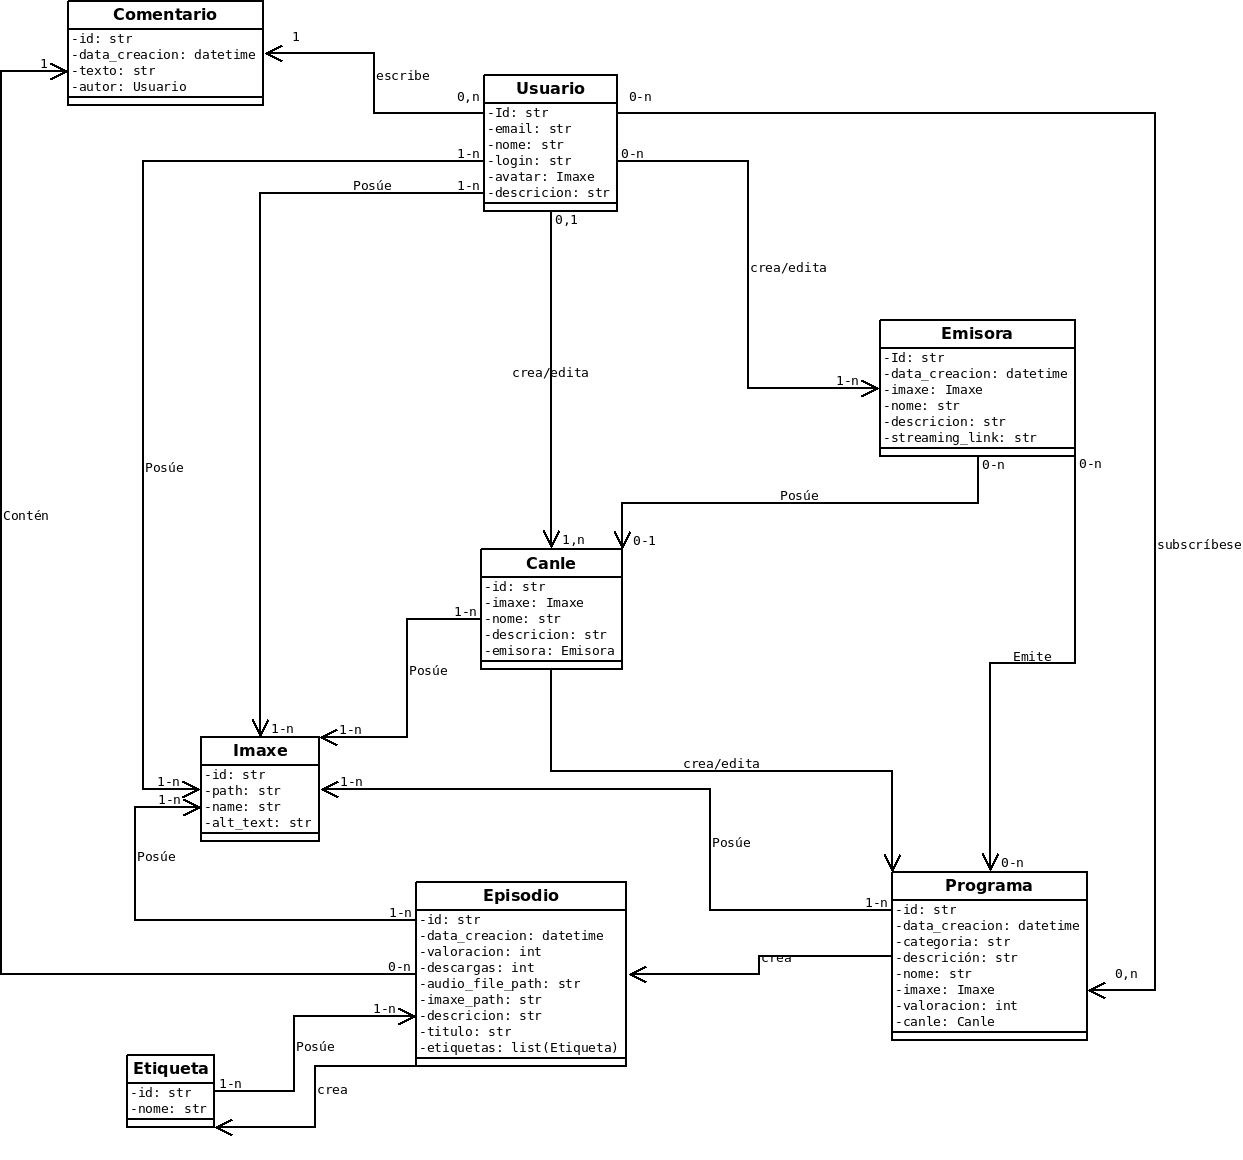
\includegraphics[scale=0.35,keepaspectratio=true]{./images/class_diagram_20171107.png}
	\caption{Diagrama de clases do primeiro borrador de deseño.}
	\label{fig:classold}
\end{figure}

Unha cousa a comentar neste primeiro modelo é a existencia dunha clase \say{canle} intermediaria entre a emisora e o programa que, como veremos, quedou finalmente desbotada. A idea era que os colectivos que realmente teñen unha emisión por onda e aqueles que publican podcasts de escoita baixo demanda terían necesidades distintas e debían diferenciarse, sempre sen bloquear a posibilidade de que unha radio emitise podcasts.

O que si previa xa este modelo era a necesidade de que os usuarios deixasen a súa impresión a cerca dos contidos, expresada no atributo \say{valoración} da clase programa. 

En canto ao RSS, fixéronse os primeiros scripts de proba utilizando a biblioteca de Python \textit{feedparser} incluída no paquete de Anaconda. Ese primeiro código era capaz de descargar un ficheiro RSS e transformalo nun obxecto cos datos do programa que á súa vez contiña unha lista de obxectos cos datos dos episodios, demostrando que a consulta de RSS si era a forma axeitada de afrontar a inserción e actualización dos contidos.

De cara a unha segunda iteración, establecéronse os seguintes obxectivos:

\begin{itemize}
	\item Instalar a infraestrutura desenvolvemento: Creación dun repositorio de control de versións (GitHub), instalación do entorno Django-PostgreSQL.
	\item Implementación de Programa e Episodio.
	\item Implementación dunha interface web básica.
\end{itemize}

\subsection{Iteración 2}